\documentclass{article}
\usepackage{graphicx}
\graphicspath{ {./} }

\title{ElasticSearch and Zipf’s and Heaps’ laws}
\date{Quadrimestre Tardor 2019 - 2020}
\author {
  Pol Renau Larrod\'e \\
  Felipe Ramis V\'asquez
}

\begin{document}
  \maketitle
  \newpage

  \section{Ley de Zipf}
        \paragraph{
            Nuestro objetivo en este apartado de la practica, es ver si una distribuci\'on de rango-frecuencia de las palabras en un gran corpus de datos, sigue la ley de la potencia.
            Con lo que tendremos que ver si  ajustando los par\'ametros de la siguiente funci\'on, encontramos una que describa a los datos, o se asemeje.
            \[ f = \frac{c}{(rank+b)^a} \]
        }
        \paragraph{
            Hemos realizado el análisis de datos sobre la colecci\'on de \textit{"corpus novels"} ya que a nuestro parecer eran los datos mas limpios.
            Indexamos todo el corpus de textos para extraer todas las palabras y sus respectivas frecuencias, usando el siguiente comando:
            \newline
            \newline
            \textit{ \$ python IndexFiles.py --index nov --path /path/to/novels}
        }
        \paragraph{
            Una vez indexado el texto limpiamos el fichero de salida, eliminando urls, fechas, palabras que contengan n\'umeros dentro o que tengan s\'imbolos no admitidos en el lenguaje.
            De esta manera tenemos una entrada limpia con la que podemos empezar a trabajar.
        }
        \paragraph{
              Realizaremos la experimentaci\'on con las 10000 palabras con la frecuencia más alta. Fijamos valores para la \textit{a}, y usamos la funci\'on de \textit{curve fit} para encontrar los valores \'optimos para b i c.
            Empezamos con 0.5, no obstante con este valor la grafica de los datos quedaba bastante por debajo que la de "fitting" ,
               as\'i que modificamos el valor de \textit{a} hasta 1.05, en este punto encontramos que la curva de "fitting" es muy parecida a la de datos.
        }
      \newpage

      \begin{figure}[!tbp]
         \begin{minipage}[b]{0.4\textwidth}
           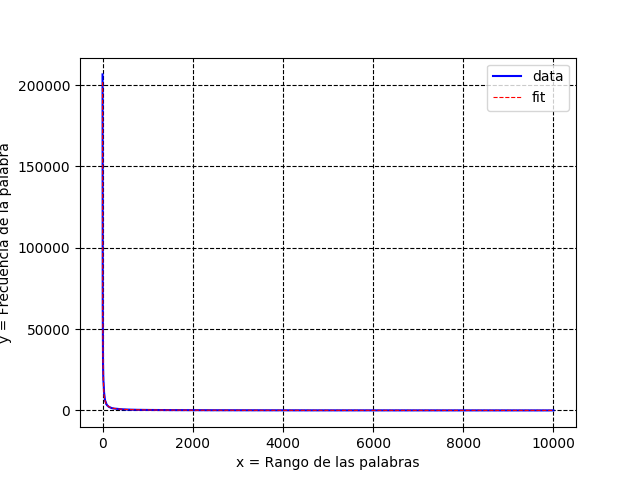
\includegraphics[width=\textwidth]{novels}
         \end{minipage}
         \hfill
         \begin{minipage}[b]{0.4\textwidth}
           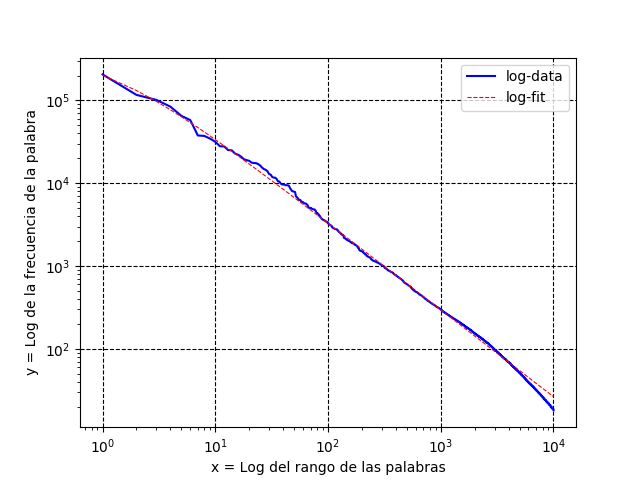
\includegraphics[width=\textwidth]{novels-Log-Log}
         \end{minipage}
      \end{figure}
      \paragraph{
        Finalmente vemos que los datos siguen la tendencia de la ley de potencia.
         Y que entonces la ley de Zipf tiene seg\'un nuestros datos una tendencia de:
         \[ f(x) = {\frac{417936}{(x+1.007)^{1.05}}} \]
       }

\newpage
  \section{Ley de Heap}
    \paragraph{
        La ley de Heap's es una ley que describe el numero total de palabras diferentes en un Documento:
        \newline
        \[d = K*N^{\beta}\]
        \newline
        d representa el numero total de palabras diferentes.
        \newline
        N representa el numero total de palabras en el documento.
        \newline
        K y ${\beta}$ s\'on par\'ametros libres.
    }
    \paragraph{
        Nuestro objetivo es encontrar un valor para K y $\beta$ para provar que se sigue la ley de Heap's.
        \newline
        Como Tenemos diferentes tama\~nos de documentos, hemos reducido el tama\~no de estos de forma iterativa, reduciendo el corupus aproximadamente para cada iteración unos 2 MB. Como el tamaño inicial del corpus es de 18MB aproximadamente, nos han salido un total de 9 \'indices diferentes.
        \newline
        Para cada indice, hemos limpiado todas las plabras que no eran v\'alidas url, n\'umeros, fechas ... hemos contabilizado el total de palabras y el total de palabras distintas.
    }
  \paragraph{
    Finalemente siguiendo la misma metodologia usada en el apartado anterior, hemos usado el metodo \textit{curve fitting}  para encontrar los valores que aproximan la ley de Heap's.
    Estos han sido los valores encontrados:
    K = 195
    $\beta$ = 0.38
  }
  \newpage
  \paragraph{
  Como podemos ver, hemos encontrado unos valores que se adaptan correctamente a nuestros datos, confirmando as\'i la ley de Heap's.
  Siguiendo la f\'ormula siguiente:
  \[d = 195*N^{0.38}\]
  }
  \begin{figure}
     \begin{minipage}[b]{0.4\textwidth}
       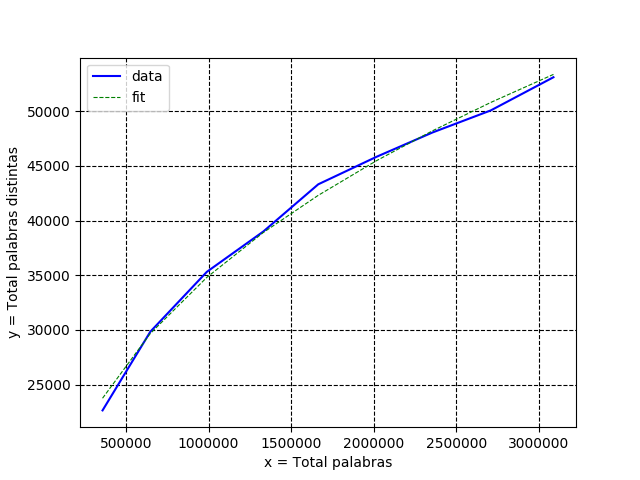
\includegraphics[width=\textwidth]{Heaps}
     \end{minipage}
     \hfill
     \begin{minipage}[b]{0.4\textwidth}
       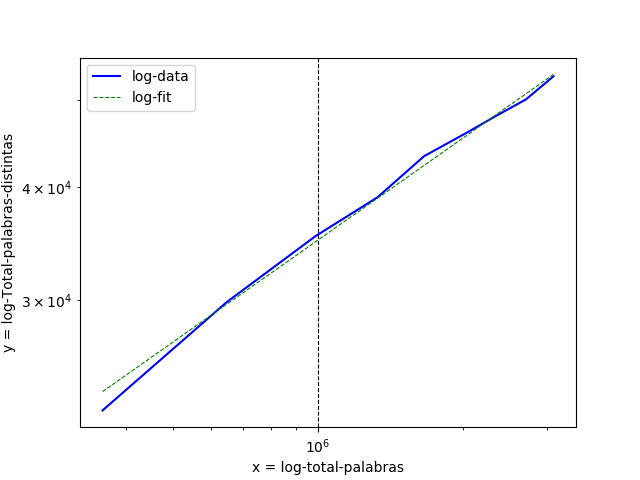
\includegraphics[width=\textwidth]{Heaps-log}
     \end{minipage}
  \end{figure}

\end{document}
